%%%%%%%%%%%%%%%%%%%%%%%%%%%%%%%%%%%%%%%%%
% Beamer Presentation
% LaTeX Template
% Version 1.0 (10/11/12)
%
% This template has been downloaded from:
% http://www.LaTeXTemplates.com
%
% License:
% CC BY-NC-SA 3.0 (http://creativecommons.org/licenses/by-nc-sa/3.0/)
%
%%%%%%%%%%%%%%%%%%%%%%%%%%%%%%%%%%%%%%%%%

%----------------------------------------------------------------------------------------
%	PACKAGES AND THEMES
%----------------------------------------------------------------------------------------

\documentclass{beamer}

\mode<presentation> {

% The Beamer class comes with a number of default slide themes
% which change the colors and layouts of slides. Below this is a list
% of all the themes, uncomment each in turn to see what they look like.

%\usetheme{default}
%\usetheme{AnnArbor}
%\usetheme{Antibes}
%\usetheme{Bergen}
%\usetheme{Berkeley}
%\usetheme{Berlin}
%\usetheme{Boadilla}
%\usetheme{CambridgeUS}
%\usetheme{Copenhagen} --
%\usetheme{Darmstadt} --
%\usetheme{Dresden}
%\usetheme{Frankfurt} --
%\usetheme{Goettingen}
%\usetheme{Hannover}
%\usetheme{Ilmenau}
%\usetheme{JuanLesPins}
%\usetheme{Luebeck}
\usetheme{Madrid}
%\usetheme{Malmoe}
%\usetheme{Marburg}
%\usetheme{Montpellier}
%\usetheme{PaloAlto}
%\usetheme{Pittsburgh}
%\usetheme{Rochester}
%\usetheme{Singapore}
%\usetheme{Szeged}
%\usetheme{Warsaw}

% As well as themes, the Beamer class has a number of color themes
% for any slide theme. Uncomment each of these in turn to see how it
% changes the colors of your current slide theme.

%\usecolortheme{albatross}
%\usecolortheme{beaver}
%\usecolortheme{beetle}
%\usecolortheme{crane}
%\usecolortheme{dolphin}
%\usecolortheme{dove}
%\usecolortheme{fly}
%\usecolortheme{lily}
%\usecolortheme{orchid}
%\usecolortheme{rose}
%\usecolortheme{seagull}
%\usecolortheme{seahorse}
%\usecolortheme{whale}
%\usecolortheme{wolverine}

%\setbeamertemplate{footline} % To remove the footer line in all slides uncomment this line
%\setbeamertemplate{footline}[page number] % To replace the footer line in all slides with a simple slide count uncomment this line

%\setbeamertemplate{navigation symbols}{} % To remove the navigation symbols from the bottom of all slides uncomment this line
}

\usepackage[spanish]{babel}
\usepackage[utf8]{inputenc}

\usepackage{graphicx} % Allows including images
\usepackage{booktabs} % Allows the use of \toprule, \midrule and \bottomrule in tables

\usepackage{subcaption}
\captionsetup{compatibility=false}

\renewcommand\footnotemark{}
\renewcommand\footnoterule{}

\usepackage[export]{adjustbox}
\usepackage{wrapfig}

\usepackage{textpos}
\usepackage{color}


\newenvironment{figure*}%
{\begin{figure}}
{\end{figure}}

%----------------------------------------------------------------------------------------
%	TITLE PAGE
%----------------------------------------------------------------------------------------

\title[RRAP]{Proyecto de grado: Routers Reconfigurables de Altas Prestaciones} % The short title appears at the bottom of every slide, the full title is only on the title page

\author{Rodrigo Amaro, Emiliano Viotti}
\institute[UdelaR] % Your institution as it will appear on the bottom of every slide, may be shorthand to save space
{
Instituto de Computaci\'on \\ Facultad de Ingeniería \\ Universidad de la República \\ \vspace{0.2cm} Tutores: Dr. Eduardo Gramp\'in, MSc. Mart\'in Giachino % Your institution for the title page
%\medskip
%\textit{john@smith.com} % Your email address
}
\date{\today} % Date, can be changed to a custom date

\begin{document}

\begin{frame}
\titlepage % Print the title page as the first slide
\end{frame}


\begin{frame}
\frametitle{Agenda} % Table of contents slide, comment this block out to remove it
\tableofcontents % Throughout your presentation, if you choose to use \section{} and \subsection{} commands, these will automatically be printed on this slide as an overview of your presentation
\end{frame}

\definecolor{blue(ryb)}{rgb}{0.01, 0.28, 1.0}

%----------------------------------------------------------------------------------------
%	PRESENTATION SLIDES
%----------------------------------------------------------------------------------------


%------------------------------------------------
\section{Introducci\'on} 
\frame{\tableofcontents[currentsection]}

\begin{frame}
\frametitle{Motivaci\'on I} 

\begin{block}{Redes acad\'emicas}
Internet no parece apropiada para su utilizaci\'on en el contexto académico en actividades de enseñanza, investigac\'on, el desarrollo de nuevos protocolos, servicios e innovaci\'on en el \'area.
\end{block}

\begin{figure}[h] 
\centering    
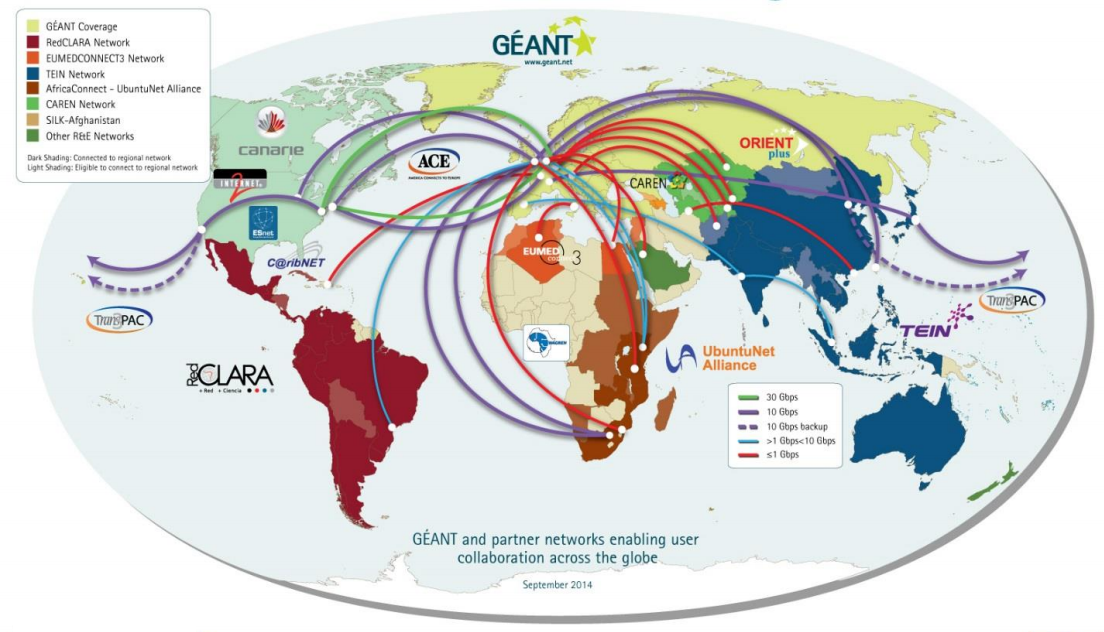
\includegraphics[width=0.7\textwidth]{imagenes/redesAcademicas.png}
\label{fig:AcademicNetworks}
\end{figure}

\end{frame}

\begin{frame}
\frametitle{Motivaci\'on II} 

\begin{block}{Red Académica Uruguaya (RAU)}
A nivel local, la RAU es un emprendimiento de la Universidad de la República administrado por el SeCIU con los objetivos de unir a las instituciones académicas nacionales en una red de alcance nacional y a trav\'es de ella conectarlas a Latinoam\'erica. 
\end{block}

\begin{block}{RAU2}
Remplazo de la actual red académica, es una red avanzada de altas prestaciones que estar\'ia dotada de funciones de virtualizaci\'on de redes flexibles en su definici\'on y uso.
\end{block}

\begin{figure}[h] 
\centering    

\includegraphics[width=0.3\textwidth]{imagenes/logorau2.png}
\label{fig:RAU}
\end{figure}

\end{frame}

\begin{frame}
\frametitle{Motivaci\'on III} 

\begin{block}{Hardware comercial}
Los equipos de red de backbone comerciales como HP, CISCO, Juniper son costosos y generalmente de naturaleza cerrada. Las funcionalidades del hardware se restringen a las funcionalidades expuestas por una API propietaria. 
\end{block}

\begin{figure}[htp]
\centering
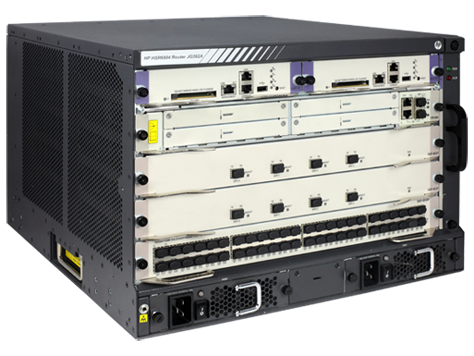
\includegraphics[width=.25\textwidth]{imagenes/corerouter2.png}\hfill
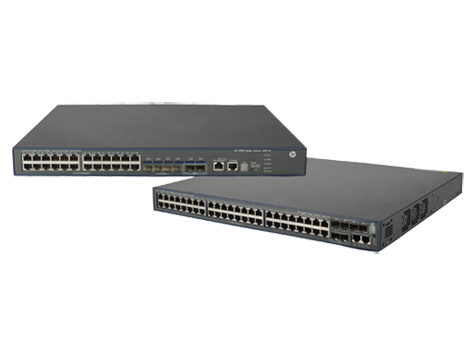
\includegraphics[width=.35\textwidth]{imagenes/corerouter1.png}\hfill
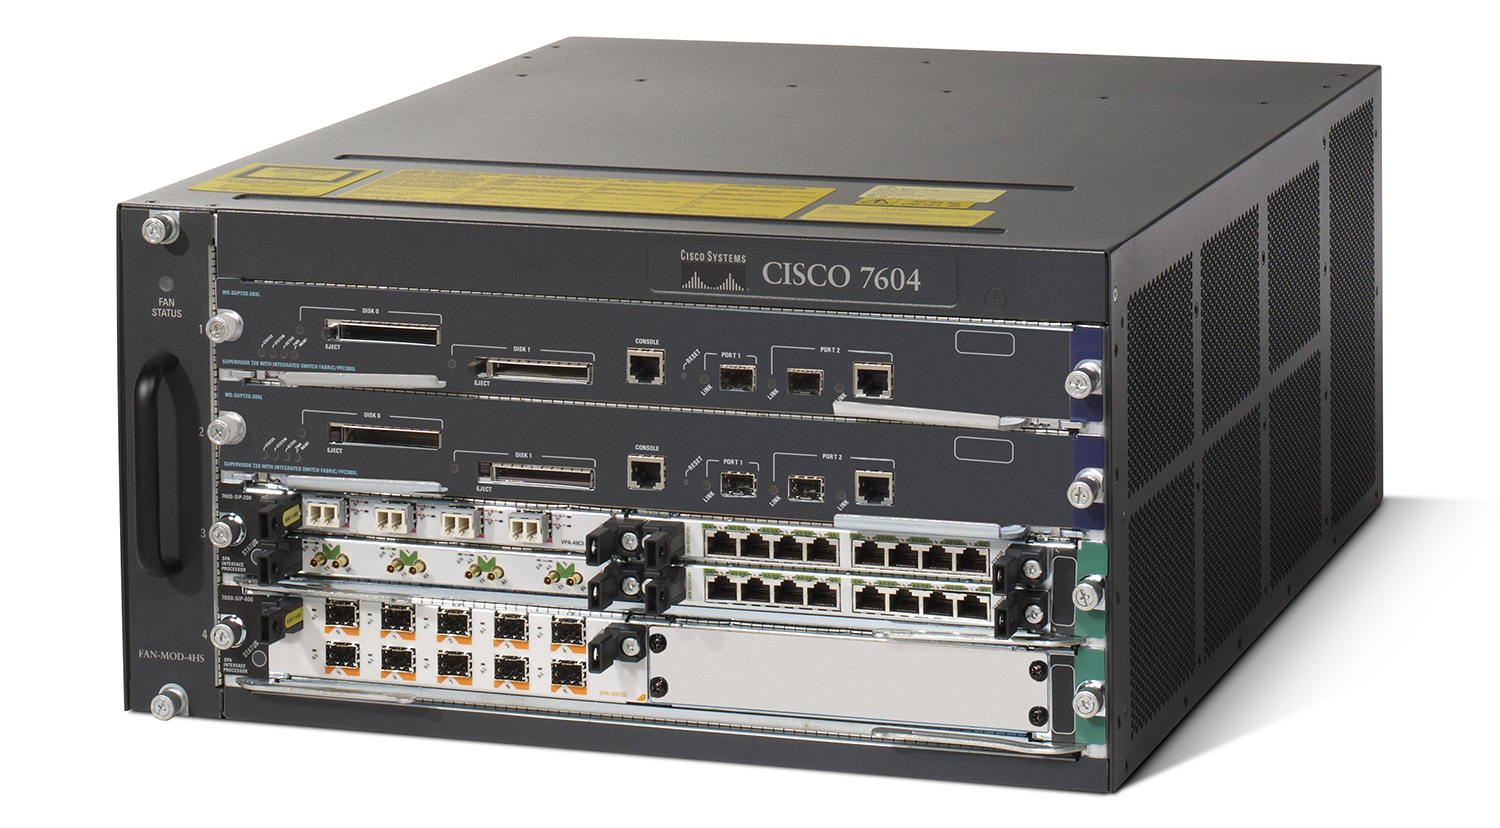
\includegraphics[width=.35\textwidth]{imagenes/corerouter3.jpg}
\label{fig:figure3}
\end{figure}
\end{frame}

\begin{frame}
\frametitle{Definición del problema I} 

\begin{block}{Definición del Problema }
Constru\'ir un prototipo para la RAU2 utilizando como plataforma PCs con placas de red aceleradas en hardware reconfigurable NetFPGA y el enfoque de las Redes Definidas por Software (SDN).
\end{block}

\pause
\begin{block}{Resultados esperados}
\begin{itemize}
\item Estado del arte en Redes Definidas por Software y hardware NetFPGA
\pause
\item Prototipo de aplicaci\'on de gesti\'on de red utilizando SDN y el hardware NetFPGA (orientado a  los requerimientos de la RAU2)
\pause
\item Diseño e implementaci\'on de pruebas funcionales
\end{itemize}
\end{block}

\end{frame}

\begin{frame}
\frametitle{Definición del problema II} 

¿Qu\'e características se esperan del prototipo, cu\'ales son los requerimientos?

\pause
{\color{blue}R: Pensemos en posibles requerimientos sobre la RAU2}

\pause
\begin{block}{Requerimientos}
\begin{enumerate}[<+->]
\item Clasificaci\'on y separaci\'on de tr\'afico seg\'un categorías
\item Manejo de grandes vol\'umenes de datos
\item Escalabilidad
%\item Red de entrega de contenidos
\end{enumerate}
\end{block}

\pause
Problema demasiado grande!\\
\pause
{\color{blue} Se hace foco en resolver (1)}

\end{frame}

%------------------------------------------------

%------------------------------------------------
\section{Conceptos preliminares} 
\frame{\tableofcontents[currentsection]}

\begin{frame}
\frametitle{Enfoque tradicional de redes} 

%SDN presenta un enfoque arquitectonico alternativo al enfoque tradicional de redes.

%Redes definidas %

	\begin{figure}[H]
		\raggedright
		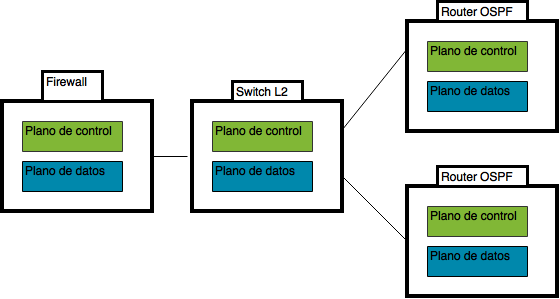
\includegraphics[width=0.5\textwidth, center]{imagenes/SDN-tradicional.png}
	\end{figure}

\hfill

%Enfoque tradicional
%La inteligencia y estado de la red se encuentra distribuida en los mismos dispositivos que reenvian la informacion

\begin{block}{Plano de control}
Es donde reside la inteligencia de la red, es la l\'ogica que controla el comportamiento de reenv\'io. Ejs : OSPF, RIP,Firewalls
%El cerebro de la red%
\end{block}



\begin{block}{Plano de datos}
Se encarga de reenviar el tr\'afico conforme a el plano de control Ejs : Reenv\'io IP
 
\end{block}


\end{frame}


\begin{frame}
\frametitle{SDN} 

\begin{block}{Definicion}

La separación física del plano de control de la red del plano de datos, donde el plano
de control controla varios dispositivos.

\end{block}

	\begin{figure}[H]
		\raggedright
		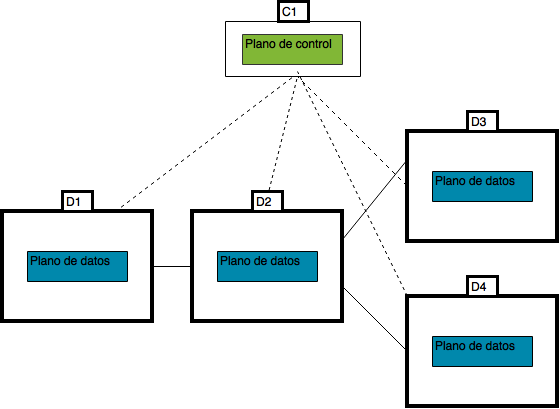
\includegraphics[width=0.5\textwidth, center]{imagenes/SDN-distribuido.png}
	\end{figure}

\end{frame}

\begin{frame}
\frametitle{SDN (Capas l\'ogicas)} 

\begin{itemize}
\item Tres capas: (1) capa de aplicaciones, (2) capa de control y (3) capa de infraestructura
\item Dos interfaces de comunicaci\'on: Interfaz Sur e Interfaz Norte
\end{itemize}
 

\begin{figure}[H]
\centering
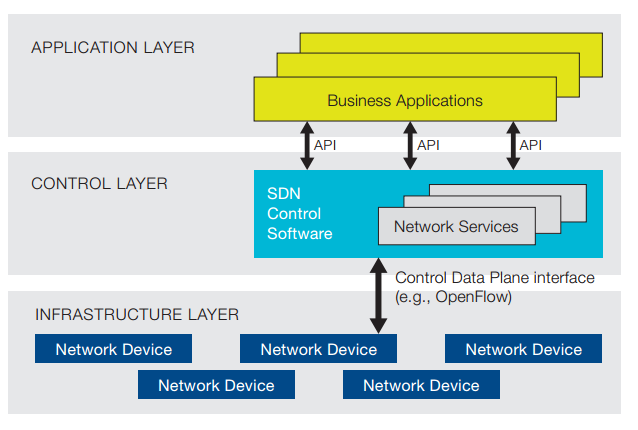
\includegraphics[width=0.6\textwidth]{imagenes/SDNArchitecture.png}
\end{figure}
\end{frame}

\begin{frame}
\frametitle{OpenFlow} 

Soluci\'on basada en el enfoque SDN, ofrece una implementaci\'on est\'andar de la Interfaz Sur. El protocolo especifica:

\begin{itemize}
\item Canal seguro de comunicaci\'on entre capa de control e infraestructura (Protocolo OpenFlow)
\item Especificaci\'on de dispositivos compatibles con la arquitectura (Switch OpenFlow)
\end{itemize}


\end{frame}

\begin{frame}
\frametitle{OpenFlow (Capa de Aplicaci\'on)} 

\begin{minipage}{0.40\textwidth}
	\begin{figure}[H]
		\centering
		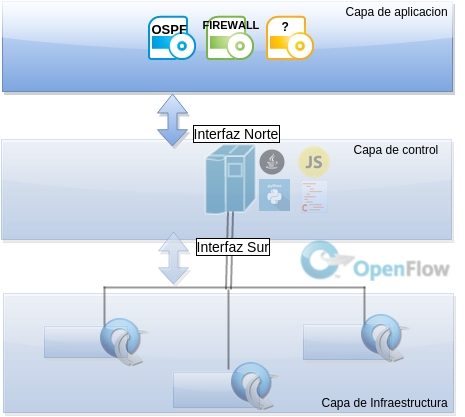
\includegraphics[width=1.0\textwidth]{imagenes/openflowApplication.png}
	\end{figure}

\end{minipage}
\hfill
\begin{minipage}{0.58\textwidth}

\begin{itemize}
\item El comportamiento de la red se implementa mediante aplicaciones
\item Se escriben en lenguajes de programaci\'on y de alto nivel (C/C++, Java, Python)
\item Se ejecutan sobre el Controlador OpenFlow y hacen uso de la API Norte
\end{itemize}

\end{minipage}

\end{frame}

\begin{frame}
\frametitle{OpenFlow (Capa de Control)} 
\begin{minipage}{0.40\textwidth}
	\begin{figure}[H]
		\centering
		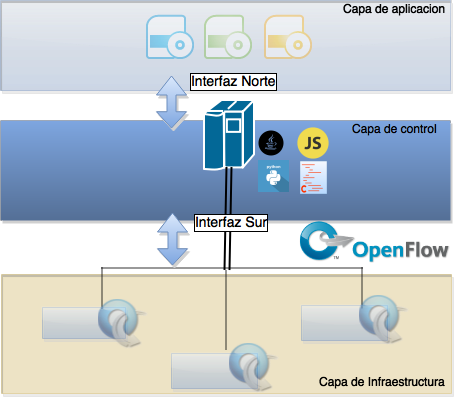
\includegraphics[width=1.0\textwidth]{imagenes/openflowController.png}
	\end{figure}
\end{minipage}
\hfill
\begin{minipage}{0.58\textwidth}
\begin{itemize}
\item Implementaci\'on en Software que se ejecuta en hardware convencional (x86)
\item Ofrece una API de alto nivel para controlar los dispositivos de una Red (Interfaz Norte)
\item Cada operaci\'on se traduce a reglas OpenFlow y comunicadas al dispositivo a trav\'es de la Interfaz Sur (protocolo OpenFlow)
\end{itemize}

\end{minipage}
\end{frame}

\begin{frame}
\frametitle{OpenFlow (Capa de Dispositivos)} 
\begin{minipage}{0.40\textwidth}
	\begin{figure}[H]
		\centering
		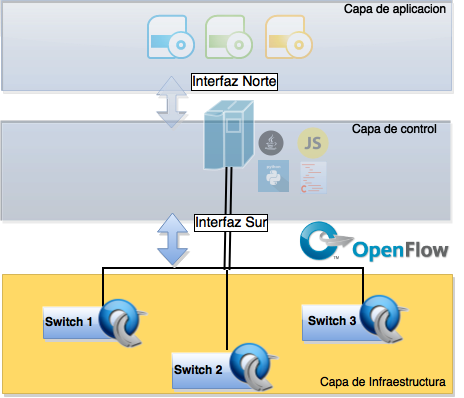
\includegraphics[width=1.0\textwidth]{imagenes/openflowDevices.png}
	\end{figure}

\end{minipage}
\hfill
\begin{minipage}{0.58\textwidth}
%Todo dispositivo OpenFlow implementa un conjunto de \textbf{Tablas de Flujos}. Mediante esta tabla se configura el plano de datos de una red. Cada entrada de esta tabla se compone de:

Cada dispositivo OpenFlow implementa \\ \textbf{Tablas de Flujos}

	\begin{figure}[H]
		\centering
		
\includegraphics[width=0.85\textwidth]{imagenes/OpenFlow.png}
	\end{figure}
 
\begin{enumerate}
\item \textbf{Regla}: Define una clase de tr\'afico
\item \textbf{Acci\'on}: Define el procesamiento (Drop, Output, Flood, GoToTable)
\item \textbf{Estad\'isticas}: Cantidad de paquetes procesados por cada flujo
\end{enumerate}
\end{minipage}

\end{frame}

\begin{frame}
\frametitle{VPN (Red Privada Virtual)} 
Extensión de una red privada sobre la infraestructura de una red pública, como por ejemplo Internet. Nos interesa diferenciarlas de acuerdo a:
\begin{itemize}
\item Que capa OSI virtualizan: L2 o L3
\item Conexi\'on utilizada: punto a punto o multipunto
\end{itemize}
	
\vspace{0.4cm}
\begin{figure}[H]
\centering
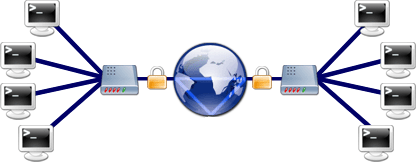
\includegraphics[width=0.65\textwidth]{imagenes/vpn.png}
\end{figure}

\end{frame}

\begin{frame}
\frametitle{MPLS} 

MPLS (Multiprotocol Label Switching) es la soluci\'on de facto para la implementaci\'on de servicios de VPN L2 y L3. Permite transportar tr\'afico mediante la conmutaci\'on de etiquetas.\\

\vspace{0.4cm}
\pause
Arquitectura:\\

\begin{itemize}
\item FEC: Clase de equivalencia de tr\'afico
\item Label: Etiqueta MPLS (20bits)
\item Acci\'on: Pop, Push y Swap
\item LSP: Camino de conmutaci\'on de etiquetas
\item LDP: Protocolo de distribución de etiquetas
\end{itemize}

\end{frame}


\begin{frame}
\frametitle{NetFPGA} 


	Plataforma de hardware de red reconfigurable y software Open Source.



%	\begin{block}{Hardware}
		Hardware: Placa PCI-E que cuenta con: 
		\begin{enumerate}
			\item Chip reconfigurable FPGA 
			\item 27Mb SRAM + 288MBytes RLDRAM
			\item 4 Puertos 10-Gigabit SFP+ Ethernet
		\end{enumerate}
		
	\begin{figure}[H]
		\centering
		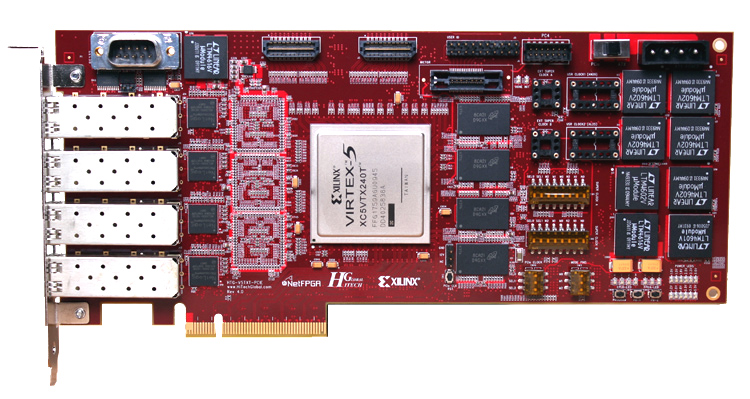
\includegraphics[width=0.65\textwidth]{imagenes/NetFPGA10G_web.jpg}
	\end{figure}

%	\end{block}

\end{frame}


\begin{frame}
\frametitle{NetFPGA} 
\begin{block}{Software}
Proyectos de software Open Source que permiten programar comportamientos en el hardware. Dos tipos de proyectos: Referencia y Comunitarios

\end{block}

\begin{table}[]
\small
\centering
\label{label}
\begin{tabular}{| p{3.7cm} | p{6.8cm} |}

\hline
\multicolumn{1}{|l|}{Proyecto \footnote[frame]{\tiny Proyectos NetFPGA extraidos de http://netfpga.org/site/\#/systems/3netfpga-10g/applications/}} & \multicolumn{1}{l|}{Organizaci\'on}\\
\hline
Production Test  & Stanford University \\
Learning CAM Switch &  Stanford University/University of Cambridge \\
Reference Router  &  Stanford University/University of Cambridge  \\
Reference NIC 10G  &  Stanford University/University of Cambridge  \\
\hline
OpenFlow Switch & Stanford University  \\
\hline  
\end{tabular}
\end{table}


\end{frame}






%------------------------------------------------
\section{Arquitectura propuesta} 
\frame{\tableofcontents[currentsection]}

\begin{frame}
\frametitle{Arquitectura propuesta I} 

\begin{itemize}
\item ¿C\'omo implementamos clasificación de tr\'afico y separamos en categorías?

\pause
{\color{blue}R: Construyendo Redes Privadas Virtuales (VPNs)}
\pause

\vspace{0.5cm}
\item ¿C\'omo implementamos Redes Privadas Virtuales?

\pause
{\color{blue}R: Utilizando MPLS (Multiprotocol Label Switching)}

\pause
\vspace{0.5cm}
\item ¿VPNs con MPLS en SDN?

\pause
{\color{blue}R: OpenFlow!}

\end{itemize}

\end{frame}


%\begin{frame}
%\frametitle{Arquitectura propuesta II} 
%
%Utilizamos OpenFlow porque:
%
%\begin{enumerate}[<+->]
%\item Es una implementaci\'on estándar y estable del enfoque SDN
%%Tiene m\'as de 7 a;os en desarrollo, se ha caracterizado por un desarrollo sostenido, ya va por la version 1.5
%\item Adopci\'on de fabricantes de hardware de red
%% Equipos comerciales lo soportan
%\item Gran variedad de software compatible
%\item Esta implementada bajo la filosofía Open Source
%\item OpenFlow incorpora soporte para MPLS desde la versi\'on 1.3.1 del protocolo
%\end{enumerate}
%
%\end{frame}
%

\begin{frame}
\frametitle{Arquitectura propuesta III} 

Se propone una arquitectura h\'ibrida que combina el enfoque SDN con tecnologías actuales, basándose 
en la implementaci\'on de OpenFlow.

\begin{figure}[H]
\centering
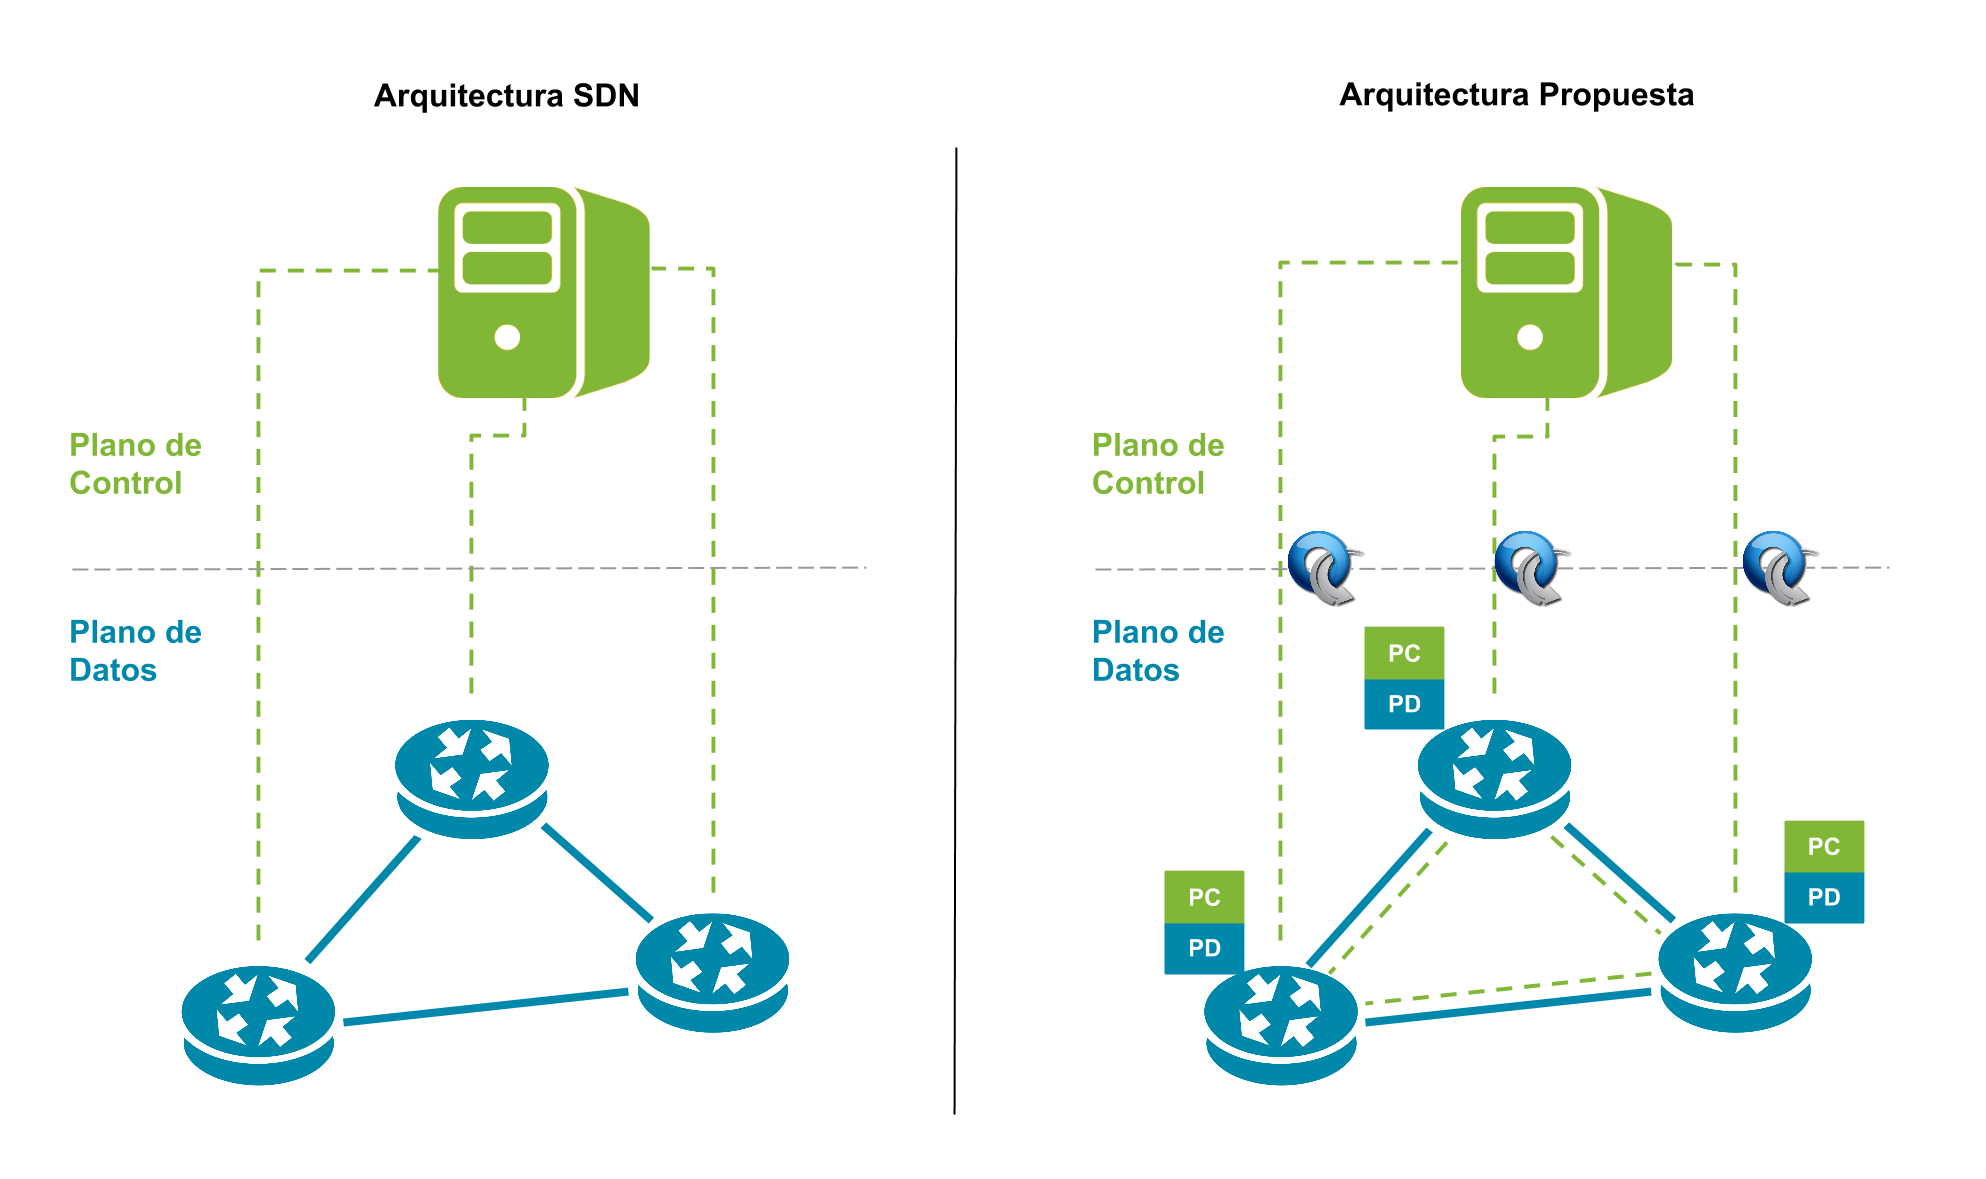
\includegraphics[width=0.95\textwidth, left]{imagenes/arquitecturapropuesta.png}
\end{figure}

\end{frame}


\begin{frame}
\frametitle{Switch OpenFlow} 

Se identifican dos alternativas utilizando hardware NetFPGA:
\pause 
\begin{enumerate}
\item Proyecto OpenFlow
\pause
\item Proyecto ReferenceNIC m\'as implementaci\'on OF en software (Open vSwitch)
\end{enumerate}

\pause
\begin{table}[]
\small
\centering
\label{label}
\begin{tabular}{| p{5cm} | p{5cm} |}

\hline
\multicolumn{1}{|l|}{(1) OpenFlow } & \multicolumn{1}{l|}{(2) ReferenceNIC y OvS } \\
\hline
Velocidad de procesamiento & Prototipaci\'on \'agil \\
Utilizaci\'on del hardaware &  Desarrollo de otras l\'ineas \\
Conocimiento espec\'ifico en HDLs &  No hay que utilizar HDLs \\
Licencias full &  Licencias econ\'omicas \\

\hline  
\end{tabular}
\end{table}

\pause
{\color{blue} (2) ReferenceNIC y OvS!}

\end{frame}

\begin{frame}
\frametitle{Controlador OpenFlow} 

Utilizamos Ryu como software de control SDN

\begin{itemize}
\item Compatible con OF hasta v1.4
\item Acad\'emico, sencillo, liviano
\item Software libre y gratuito
\end{itemize}

\begin{figure}[H]
\centering
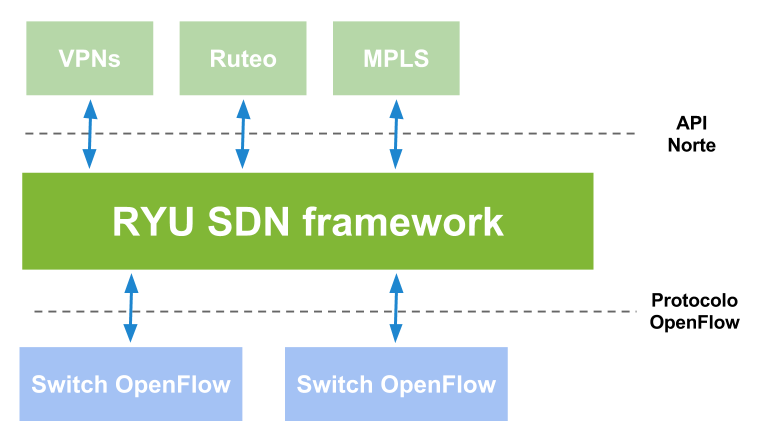
\includegraphics[width=0.65\textwidth]{imagenes/ryuarch.png}
\end{figure}

\end{frame}

\begin{frame}
\frametitle{Algoritmo de Ruteo} 

\begin{itemize}
\item Calculo de rutas en base a IP
\item Utilizamos OSPF para la construcci\'on de una base de datos topol\'ogica (LSDB)
\item Cada nodo en la red incluyendo el controlador ejecutan un demonio OSPF de la herramienta Quagga
\item Algoritmo de ruteo como App SDN en el controlador, toma informaci\'on de la LSDB
\end{itemize}

\end{frame}

%\begin{frame}
%\frametitle{Agente SNMP} 
%
%\textbf{Agente SNMP} \\
%OpenFlow no prev\'e un mecanismo para informar al plano de control direccionamiento IP de un puerto en un dispositivo. \\
%
%\vspace{0.5cm}
%\textbf{Soluci\'on:}  Utilizamos un agente SNMP en cada nodo de la red para obtener mapeo entre puertos OF y direcciones IP
%
%\end{frame}

\begin{frame}
\frametitle{Arquitectura Propuesta III} 

\begin{figure}[H]
\centering
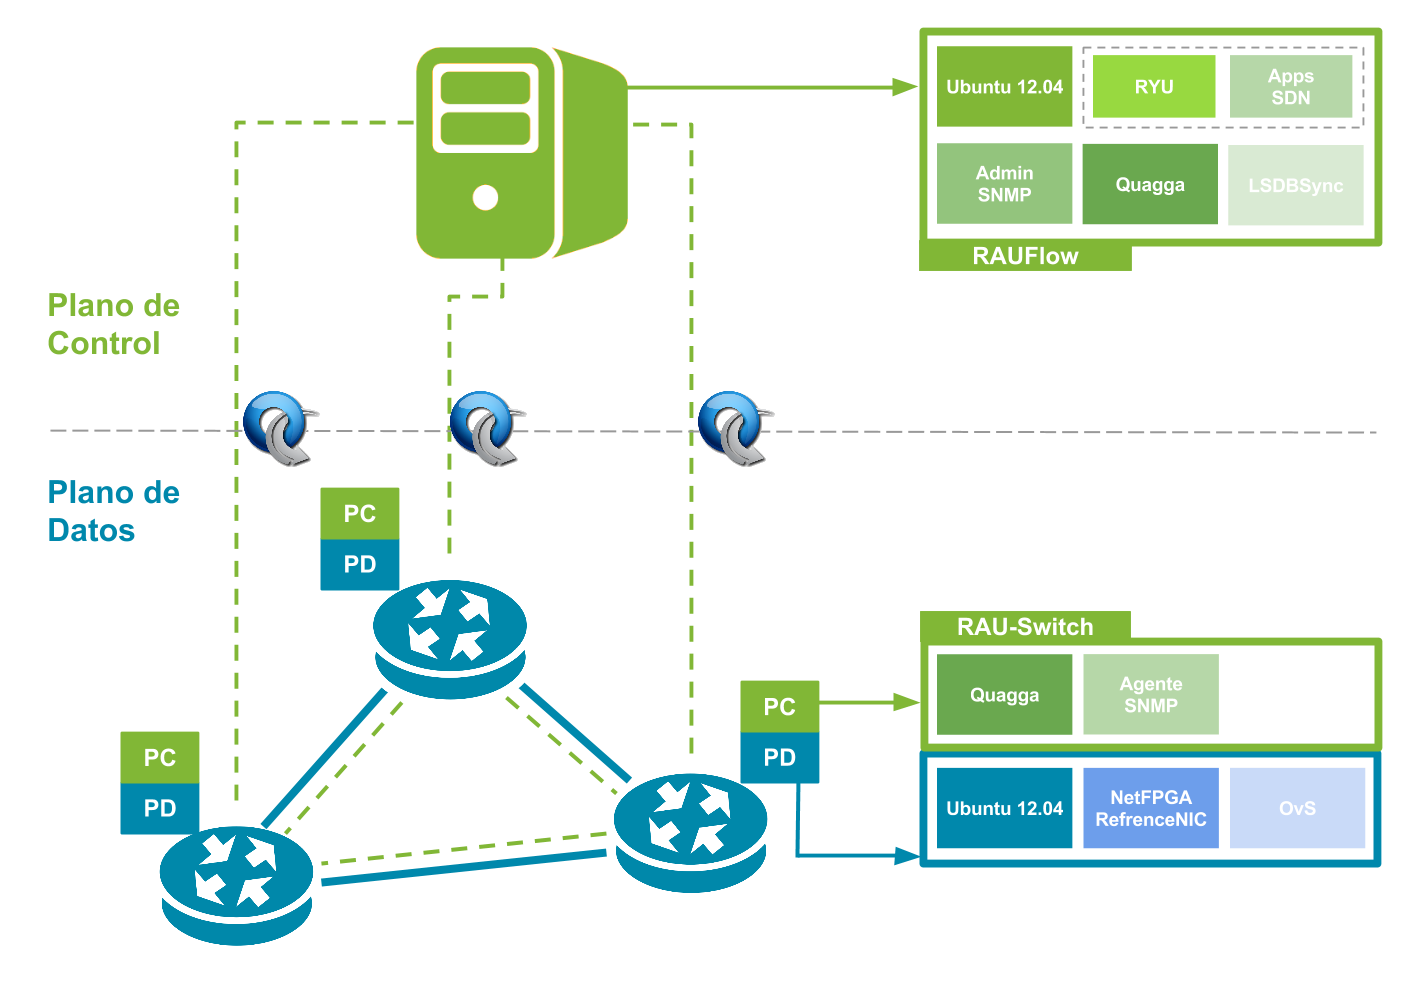
\includegraphics[width=0.80\textwidth]{imagenes/arquitecturapropuesta1.png}
\end{figure}

\end{frame}

%------------------------------------------------

%------------------------------------------------
\section{Implementaci\'on} 
\frame{\tableofcontents[currentsection]}

%\begin{frame}
%\frametitle{Implementaci\'on I} 
%
%Se implementaron dos componentes:
%
%\begin{enumerate}
%\item RAU-Switch: Dispositivo de red compatible con el protocolo OpenFlow
%\item RAUFlow: Conjunto de aplicaciones de gesti\'on de redes, implementan plano de control en el prototipo
%\end{enumerate}
%\end{frame}

\begin{frame}
\frametitle{Algoritmo de ruteo} 

\textbf{SPF(Shortest Path First):} Algoritmo del camino m\'as corto utilizando el algoritmo Dijkstra generalizado para multigrafos dirigidos\footnote[frame]{\tiny Implementaci\'on basada en "Generalization of dijkstra's algorithm for extraction of the shortest paths in directed multigraphs".}.

\begin{figure}[H]
\centering
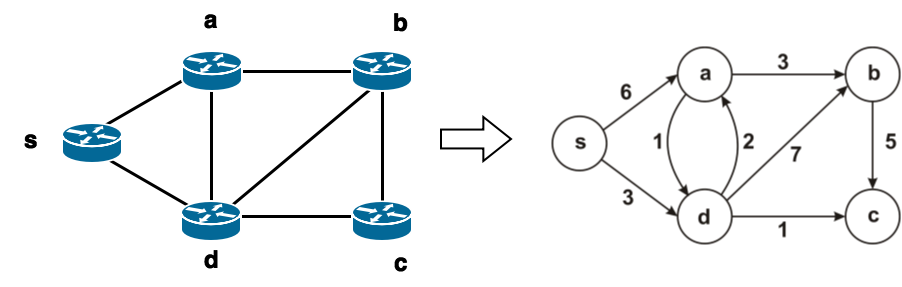
\includegraphics[width=0.85\textwidth]{imagenes/dijkstraRed.png}
\end{figure}

\pause
\textbf{CSPF(Constrained Shortest Path First):} Algoritmo SPF con restricciones.

\end{frame}

\begin{frame}
\frametitle{Clasificaci\'on de tr\'afico} 

\begin{itemize}
\item Se implementa clasificaci\'on de tr\'afico utilizando matching fields OF en los nodos de ingreso a la red
\item Cada definici\'on de servicio define una FEC que se traduce a un flujo OpenFlow para la clasificaci\'on de tr\'afico
\end{itemize}

\vspace{0.3cm}

\begin{minipage}{0.40\textwidth}

\begin{figure}[htp]
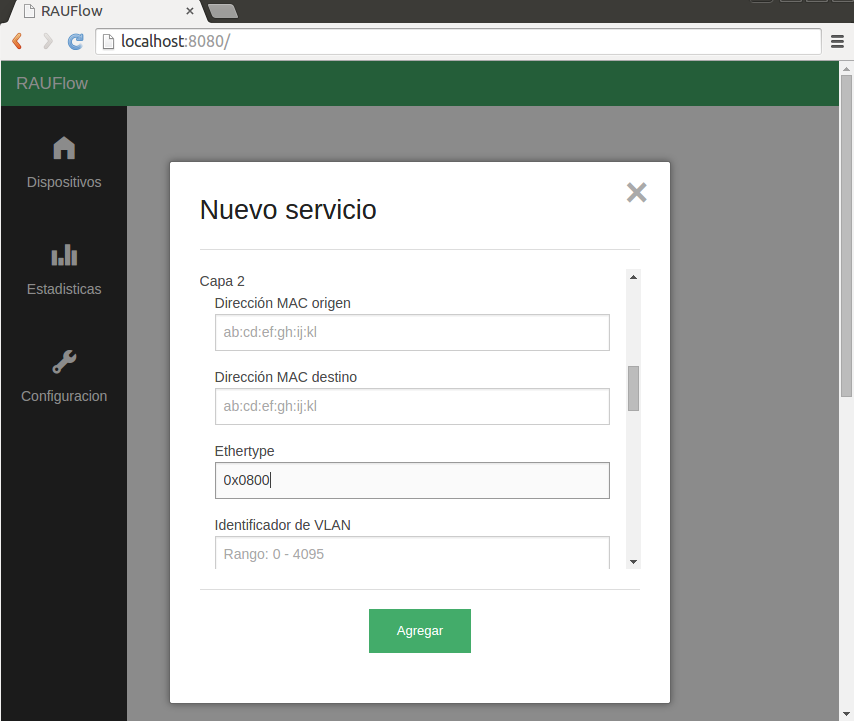
\includegraphics[width=1.0\textwidth]{imagenes/rauflowsnap.png}
\end{figure}

\end{minipage}
\hfill
\begin{minipage}{0.59\textwidth}
\centering
\begin{figure}[htp]
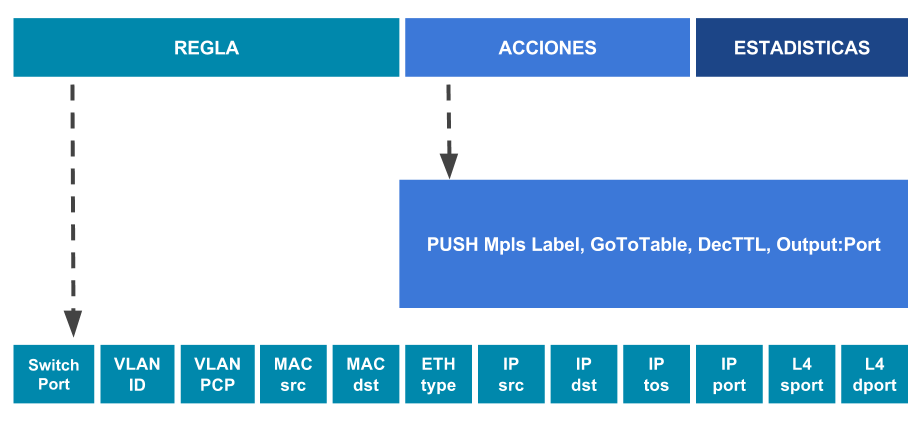
\includegraphics[width=1.0\textwidth]{imagenes/clasificaciontra.png}
\end{figure}

\end{minipage}



\end{frame}

\begin{frame}
\frametitle{RAUFlow} 

\begin{figure}[H]
\centering
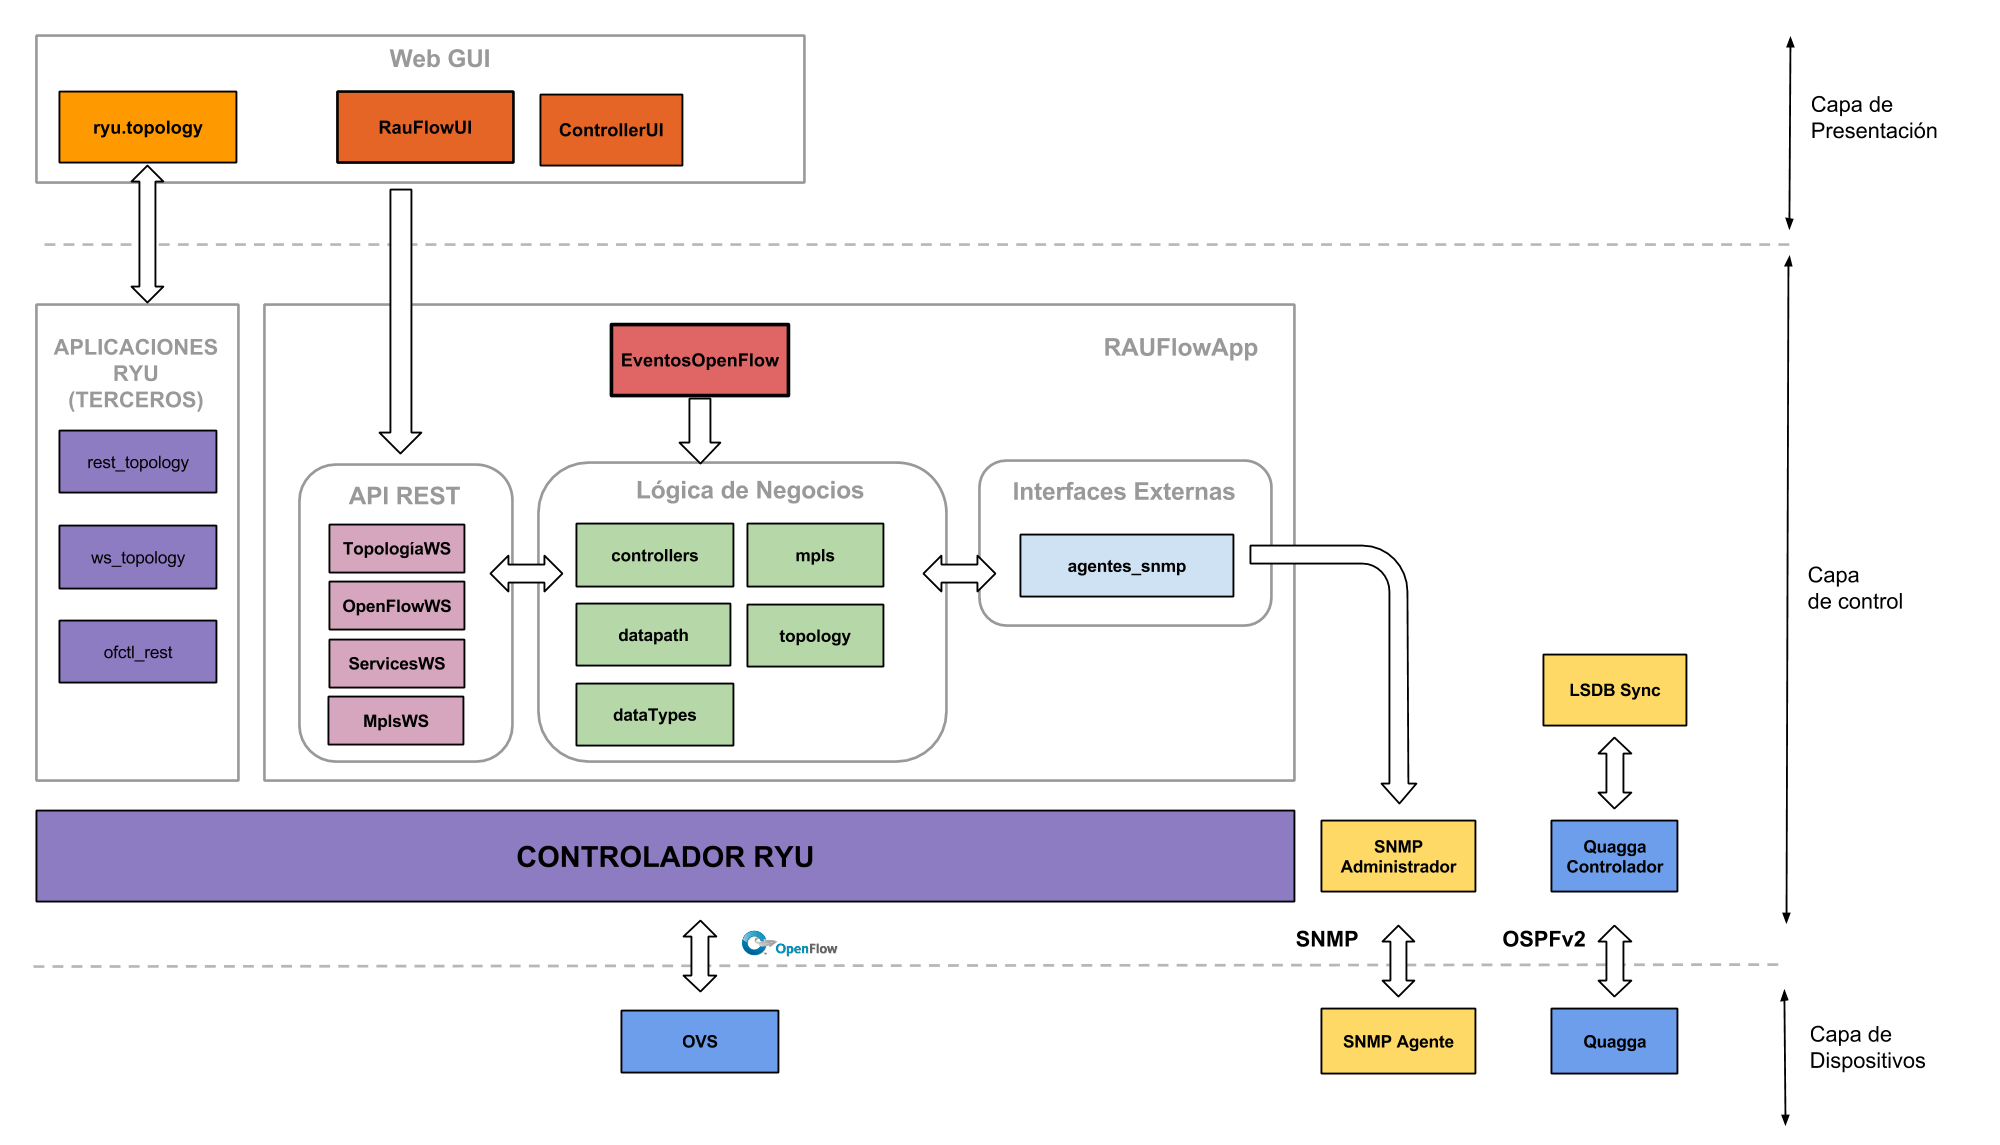
\includegraphics[width=1.0\textwidth]{imagenes/rauflowarquitectura.png}
\end{figure}

\end{frame}
%------------------------------------------------

%------------------------------------------------
\section{Experimentaci\'on} 
\frame{\tableofcontents[currentsection]}

\begin{frame}
\frametitle{Experimentaci\'on} 

Se construye un laboratorio de experimentaci\'on compuesto por 4 nodos RAU-Switch conectados mediante enlaces \'opticos de alta velocidad en una topolog\'ia full Mesh.

\vspace{0.5cm}
\begin{minipage}{0.60\textwidth}
\begin{figure}[htbp]
\centering
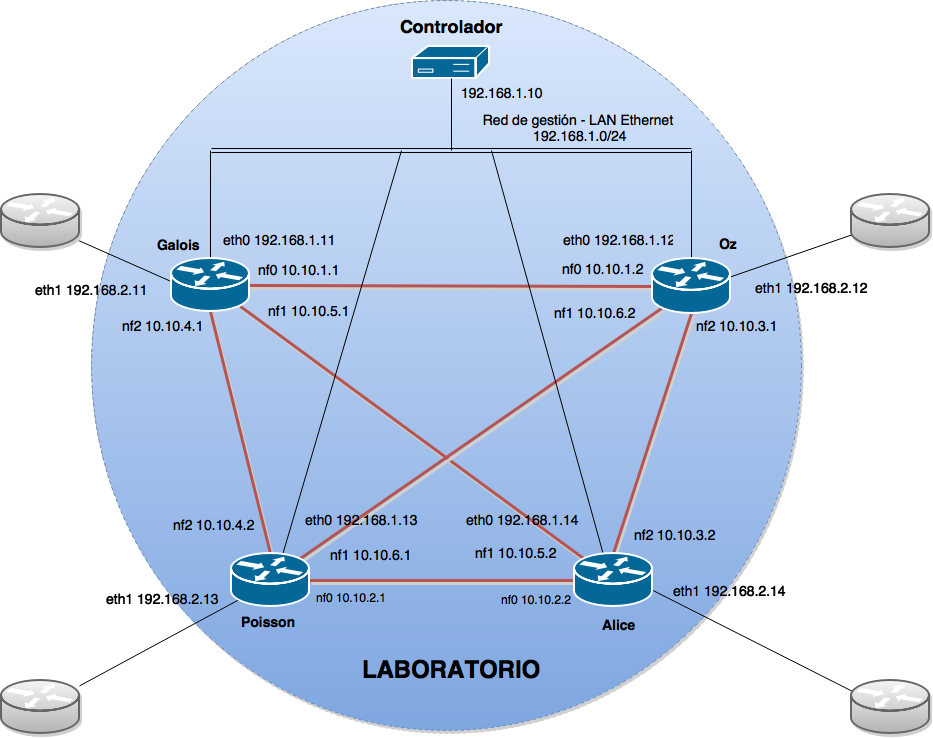
\includegraphics[width=0.81\textwidth]{imagenes/Topologia.png}
\end{figure}
\end{minipage}
\hfill
\begin{minipage}{0.35\textwidth}
\begin{figure}[H]
\centering
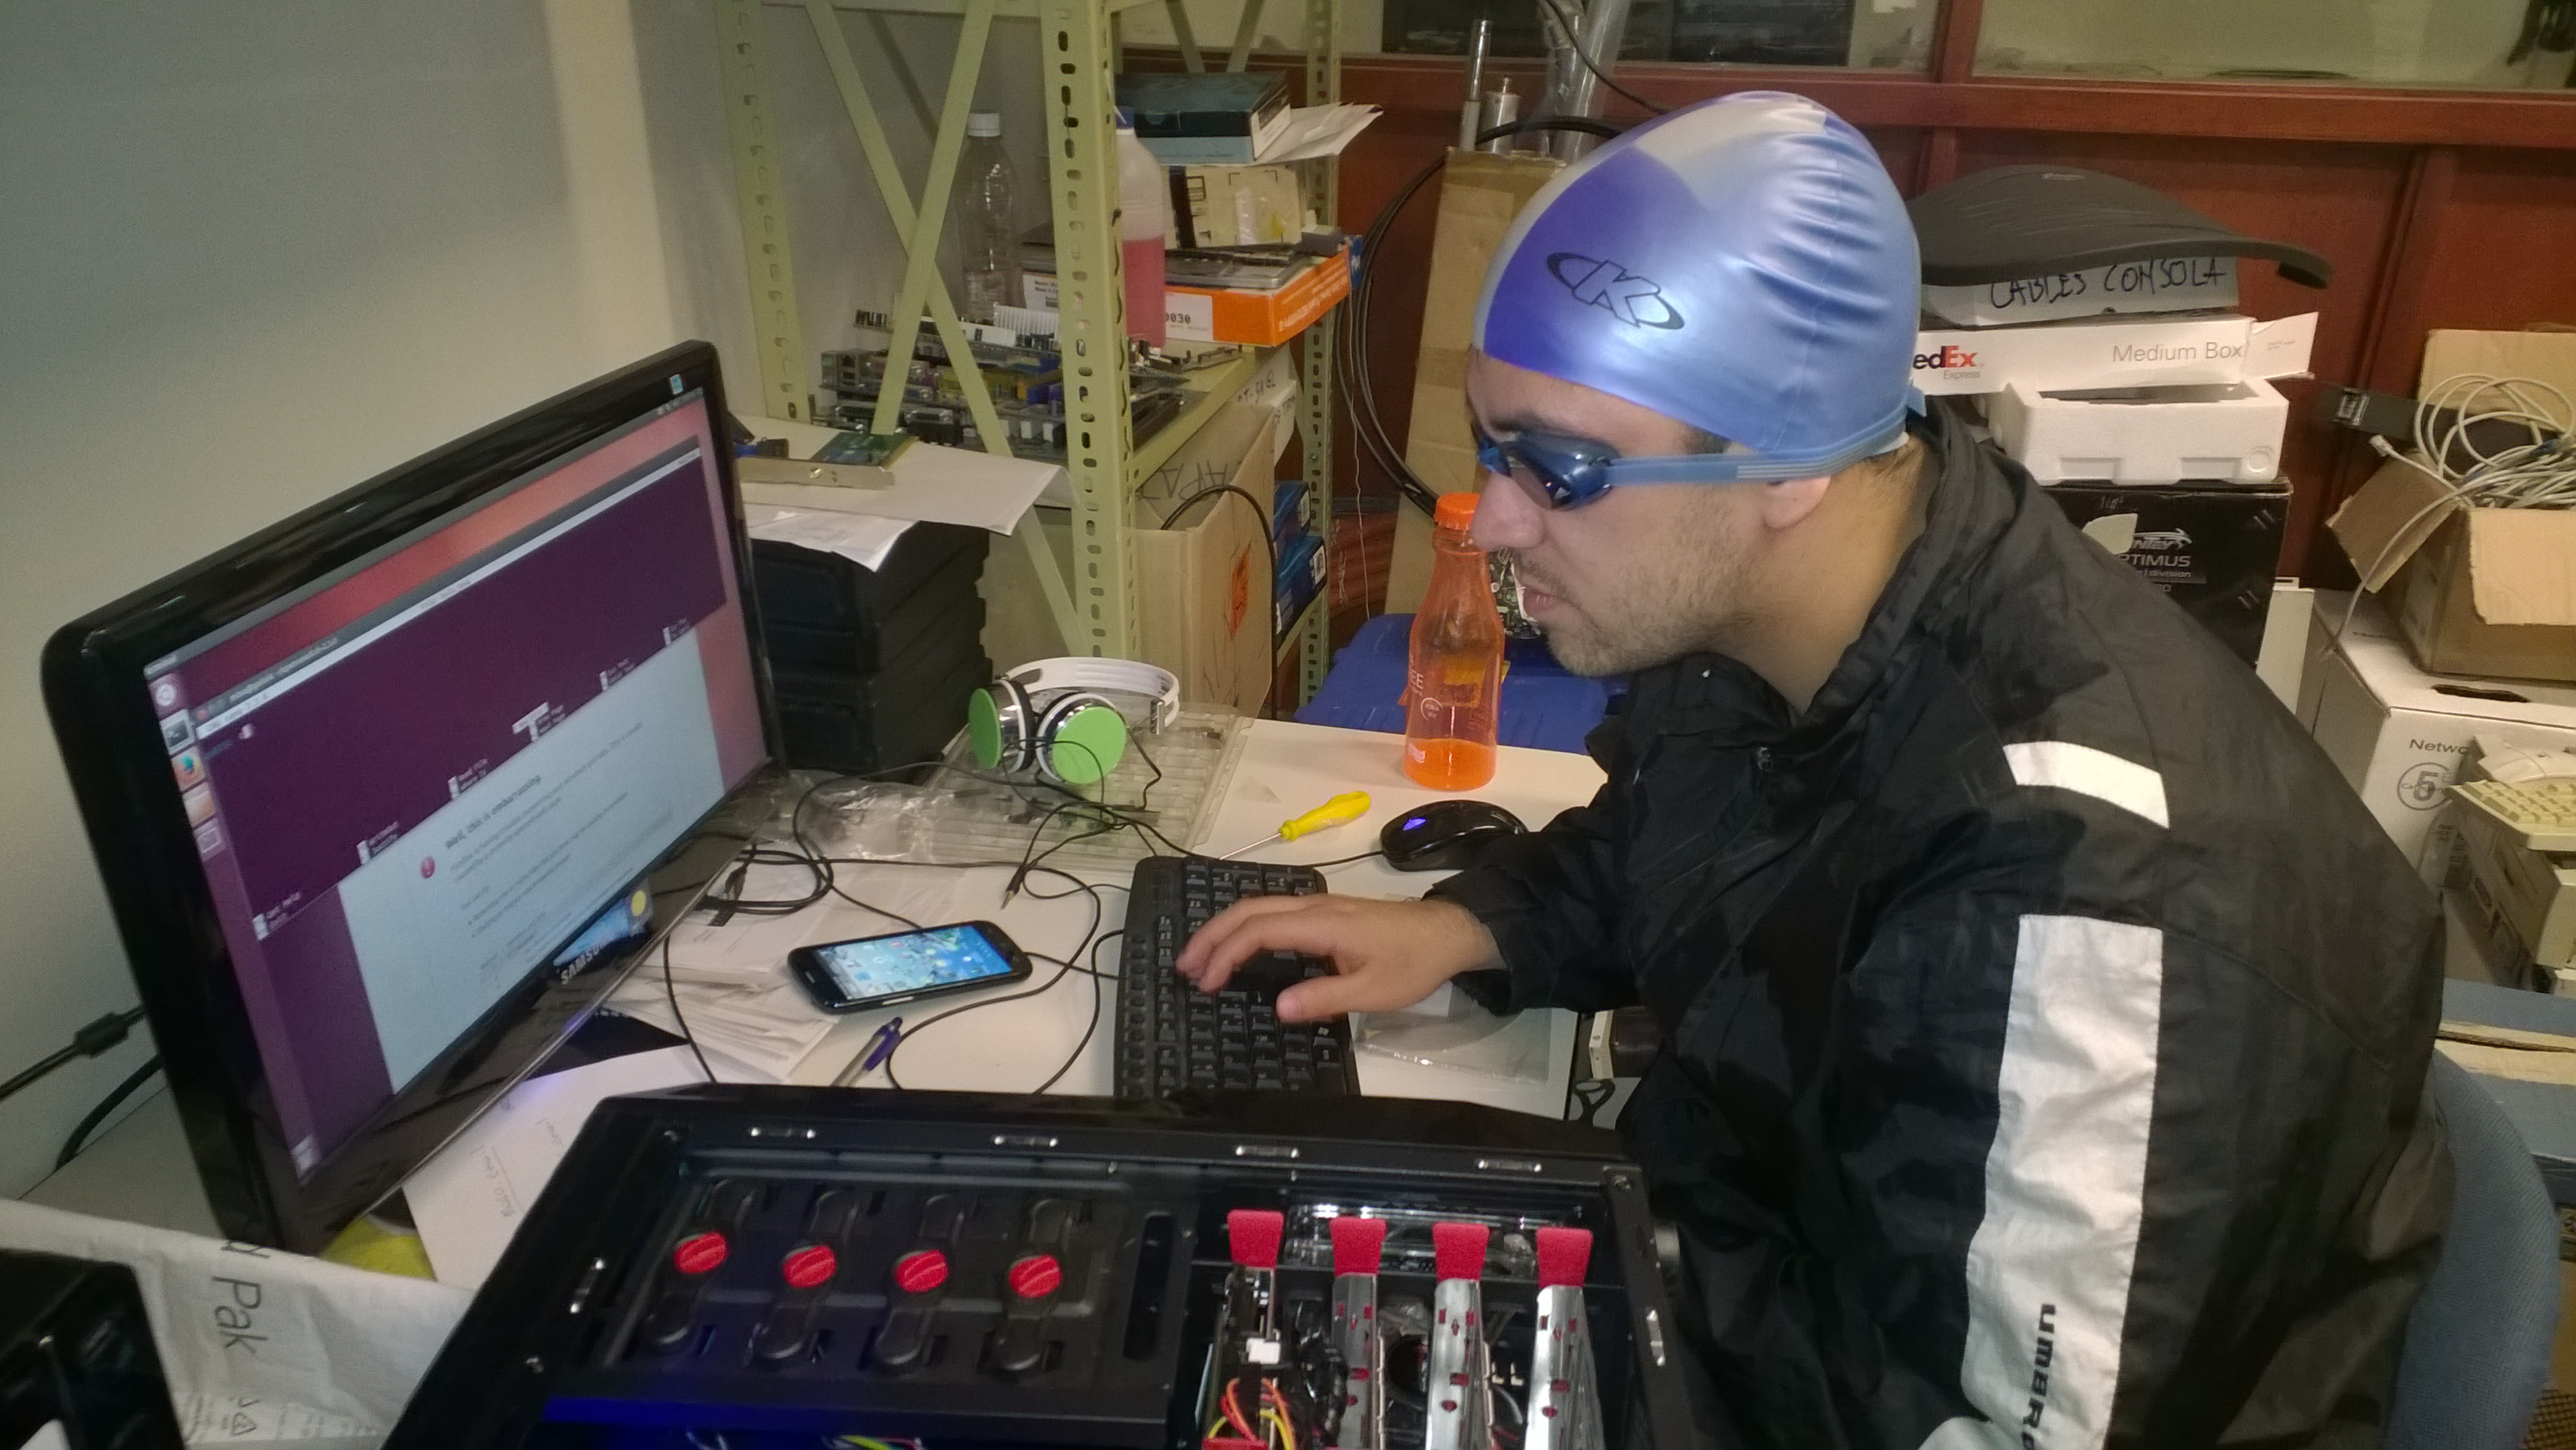
\includegraphics[width=1.0\textwidth]{imagenes/laboratorio.jpg}
\end{figure}
\end{minipage} 

\end{frame}

%\begin{frame}
%\frametitle{VPN L3} 
%
%Se configuraron dos escenarios diferentes de VPN L3:
%
%\begin{enumerate}
%\item E1: Una organizaci\'on con tres sucursales f\'isicamente separadas (VPN Multipunto)
%\item E2: Dos organizaciones con dos sucursales f\'isicamente separadas (VPN Punto a Punto)
%\end{enumerate}
%
%\vspace{0.4cm}
%
%Se crearon los servicios de VPN y se verific\'o:
%\begin{itemize}
%\item Aislamiento del espacio de direcciones IP
%\item Correcta clasificaci\'on de tr\'afico
%\item Definici\'on de servicios mediante OF Matching Fields
%\end{itemize}
%
%
%\end{frame}

\begin{frame}
\frametitle{Experimentaci\'on II} 

\textbf{Objetivos:}
\begin{enumerate}
\item Comprobar funcionalmente la implementaci\'on realizada:
\begin{itemize}
\item Algoritmo de ruteo
\item Algoritmo LDP
\item Clasificaci\'on de tr\'afico
\end{itemize}
\item Validar la aplicabilidad del enfoque SDN en la construcci\'on de un prototipo para la RAU2:
\begin{itemize}
\item VPN L3
\item VPN L2
\end{itemize}
\end{enumerate}
\end{frame}

\begin{frame}
\frametitle{VPN L3 Escenario 1} 

Se configur\'o una VPN L3 multipunto conectando 3 sucursales f\'isicamente separadas de una misma organizaci\'on.

\begin{figure}[H]
\centering
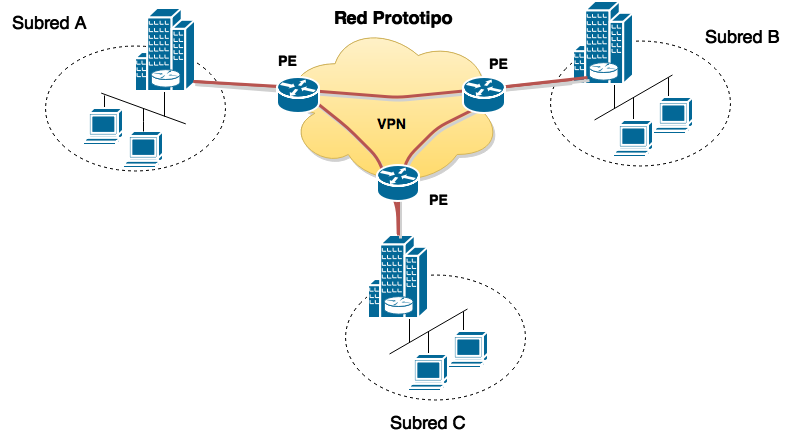
\includegraphics[width=0.5\textwidth]{imagenes/VPNMultipunto.png}
\end{figure}

Sobre este escenario se verific\'o:
\begin{itemize}
\item Correcto enrutamiento a cada sucursal de la organizaci\'on
\item Correcta clasificaci\'on de tr\'afico
\item Definici\'on de servicios mediante OF Matching Fields
\end{itemize}

\end{frame}

\begin{frame}
\frametitle{VPN L3 Escenario 2} 

Se configuraron dos VPN L3 punto a punto conectando para dos organizaciones distintas y con la misma numeraci\'on IP en sus red, dos sucursales f\'isicamente separadas. 

\begin{figure}[H]
\centering
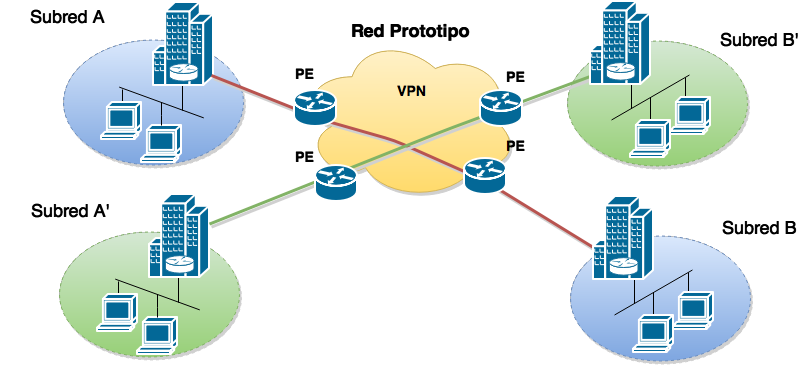
\includegraphics[width=0.5\textwidth]{imagenes/VPNPPE1.png}
\end{figure}

Sobre este escenario se verific\'o:
\begin{itemize}
\item Aislamiento del espacio de direcciones IP
\end{itemize}


\end{frame}


\begin{frame}
\frametitle{VPN L2} 

Se configur\'o una VPN L2 punto a punto para una organizaci\'on con dos sucursales f\'isicamente separadas.

\begin{figure}[H]
\centering
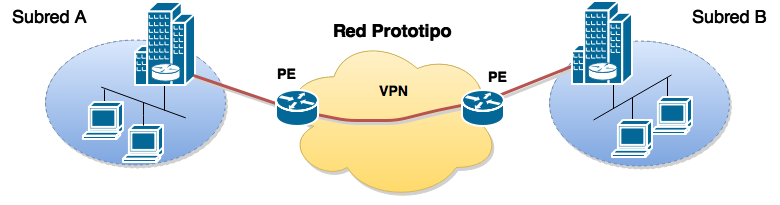
\includegraphics[width=0.5\textwidth]{imagenes/VPNL2.png}
\end{figure}

Sobre este escenario se verific\'o:
\begin{itemize}
\item Soporte para un conjunto de 43 ethertypes diferentes independiente de la definici\'on del servicio
\item En particular los protocolos ARP, IPv4 IPv6 e IP con tags de VLAN
\end{itemize}


\end{frame}
%------------------------------------------------

%------------------------------------------------
\section{Conclusiones} 
\frame{\tableofcontents[currentsection]}

%\begin{frame}
%\frametitle{Conclusiones} 
%
%\begin{itemize}
%\item Se realiz\'o una investigaci\'on en profundidad del estado del arte de las redes definidas por software (SDN) y la plataforma de hardware NetFPGA.
%\end{itemize}
%\end{frame}

\begin{frame}
\frametitle{Conclusiones I} 

Se alcanzaron los objetivos planteados al inicio del proyecto: 
\begin{itemize}[<+->]

\item Se explor\'o la aplicabilidad del enfoque SDN y el hardware NetFPGA para la construcci\'on de un prototipo para la RAU2

\item Se propuso una arquitectura h\'ibrida entre el paradigma de redes actual y el enfoque OpenFlow/SDN

\item Se construy\'o un Router IP/MPLS libre y de c\'odigo abierto sin la complejidad de la implementaci\'on de MPLS-Linux

\item Se implement\'o un prototipo de aplicaci\'on de control y gesti\'on de red utilizando SDN (RAUFlow) 

\item Se construy\'o un laboratorio de pruebas e implement\'o un par de casos de uso representativos para la RAU2

\end{itemize}
\end{frame}


\begin{frame}
\frametitle{Conclusiones II} 

Se obtuvieron resultados interesantes:
\begin{itemize}[<+->]
\item Se confeccion\'o un manual para la construcci\'on del dispositivo RAU-Switch

\item Se contribuy\'o a la comunidad NetFPGA reportando dos errores

\item Se escribió un articulo cient\'ifico el cual fue aceptado en la conferencia Latin American Network Operations and Management Symposium 2015 (LANOMS)

\item Se gener\'o un grupo de trabajo (GT SDNUY) uniendo profesionales del SeCIU, del Centro de Capacitación y Desarrollo de ANTEL y del Centro Universitario de la Región Este (CURE) 

\end{itemize}

\end{frame}

%Se implement ́o un prototipo de red de backbone utilizando el
%hardware NetFPGA y el enfoque SDN
%Se implement ́o un conjunto de pruebas para la verificaci ́on del
%prototipo construido

%------------------------------------------------

%------------------------------------------------
\section{Trabajo a futuro} 
\frame{\tableofcontents[currentsection]}

\begin{frame}
\frametitle{Trabajo a futuro} 

Se identifican las siguientes l\'ineas de trabajo a futuro:
\pause

\begin{itemize}[<+->]

\item Extender el proyecto OpenFlow de la plataforma NetFPGA para soportar al menos la versi\'on 1.3.1 del protocolo OpenFlow

\item Extender el algoritmo de ruteo SPF para implementar un CSPF

\item Incorporar en RAUFlow la capacidad de soportar m\'ultiples caminos para un mismo Servicio,  balanceo de carga, QoS e Ingenier\'ia de tr\'afico (evaluando las limitantes de Open vSwitch)

\end{itemize}

\end{frame}

\begin{frame}
\frametitle{Trabajo a futuro} 

Otras posibles l\'ineas:
\pause
\begin{itemize}[<+->]

\item Agregar una capa de persistencia para ciertos datos

\item Investigar la escalabilidad de RAUflow en topolog\'ias de red realistas 

\item Construir una jerarqu\'ia de controladores e investigar el impacto en el rendimiento 

\item Incorporar m\'as dimensiones a la definici\'on de un servicio (tiempo)

\end{itemize}

\end{frame}

\begin{frame}
\centering
\Huge
¿Preguntas?

\end{frame}

%------------------------------------------------

%----------------------------------------------------------------------------------------

\end{document} 

